\documentclass[a4paper]{article}
\usepackage[french]{babel}
\usepackage{url,graphicx,hyperref}
\usepackage{color}
\definecolor{grey}{rgb}{0.95,0.95,0.95}
\definecolor{keyword}{rgb}{0,0,0.95}
\definecolor{comment}{rgb}{0.95,0,0}
%\definecolor{include}{rgb}{0.55,0,0}
\definecolor{string}{rgb}{0,0.55,00.95}

\usepackage{listings}
\lstset{backgroundcolor=\color{grey},
        language=C, 
        numbers=left,
        numbersep=6pt,
        basicstyle=\small\ttfamily,
        extendedchars=true,
        tabsize=3,
        keywordstyle=\color{keyword}\bfseries,
        commentstyle=\color{comment},
%       includestyle=\color{include},
        stringstyle=\color{string}\itshape,
        columns=fullflexible,
        keepspaces=true
}
\usepackage{geometry}
\geometry{verbose,a4paper,tmargin=2.5cm,bmargin=2cm,lmargin=2cm,rmargin=1cm}

\begin{document}
\begin{center}
{\bf\Large Utilisation d'un simulateur de processeur}\\
\'E. Carry, J.-M Friedt, \today
\end{center}

Nous allons profiter de l'incapacit\'e de nous rencontrer pour exploiter
un simulateur de processeur pour aboutir dans la r\'ealisation du projet
de commande d'un oscillateur \`a quartz pour l'asservir sur le 1-PPS de
GPS.

\section{Introduction}

Nous avions discut\'e dans \cite{emu} de l'utilisation d'un \'emulateur
d'Atmega32U4 libre nomm\'e {\tt simavr} 
\footnote{\url{https://github.com/buserror/simavr} et son excellente 
documentation \`a \url{https://polprog.net/papiery/avr/simavr.pdf}}, outil 
capable d'ex\'ecuter un code compil\'e pour une cible -- Atmega, ARM ou RISC-V 
dans le cas de cet article -- autre que l'architecture de l'h\^ote sur lequel 
nous travaillons -- g\'en\'eralement un PC bas\'e sur un processeur compatible 
x86. Cette m\'ethode de travail a l'avantage de permettre d'appr\'ehender du 
mat\'eriel que nous ne poss\'edons pas, d'\'emuler le comportement de 
p\'eriph\'eriques en cours de d\'eveloppement ou simplement de pallier 
l'absence de mat\'eriel comme c'est le cas ici.

Dans \cite{emu}, nous avions \'et\'e dans l'incapacit\'e d'\'emuler le 
comportement du mat\'eriel autour du c\oe ur du microcontr\^oleur et nous 
\'etions content\'e d'observer le comportement du processeur ex\'ecutant des 
instructions, communiquant par UART ou manipulant ses GPIO par l'affichage de 
chronogrammes. Nous allons ici compl\'eter cette \'emulation en ajoutant les 
p\'eriph\'eriques entourant l'Atmega32U4 pour permettre d'achever le projet 
que nous avons commenc\'e. Il nous faut donc \'emuler un signal 1-PPS (issu 
normalement du r\'ecepteur GPS) pour alimenter l'entr\'ee {\em input capture} 
d'un timer, et r\'ecup\'erer la sortie PWM pour ajuster la fr\'equence du 
quartz.

\noindent\fbox{\parbox{\linewidth}{La compilation de {\tt simavr} s'obtient 
trivialement en clonant le d\'ep\^ot {\tt git} et par {\tt make} dans le 
r\'epertoire ainsi cr\'e\'e. On prendra cependant soin de cloner l'exemple 
propos\'e dans \url{https://github.com/jmfriedt/l3ep/} et de copier 
{\tt board\_project} \`a c\^ot\'e des autres exemples de {\tt examples/} 
{\bf avant} cette premi\`ere compilation. Noter que le nom du r\'epertoire 
importe car le {\tt Makefile} de {\tt examples} ne compile que le contenu 
des r\'epertoires dont le nom commence par {\tt board} 
({\tt for bi in \$\{boards\}; do ...}).}}

Une fois {\tt simavr} compil\'e, nous trouvons dans {\tt simavr/} le programme 
{\tt run\_avr} qui prend comme argument le firmware (ex\'ecutable binaire au 
format ELF) tel que nous avions l'habitude de le compiler pour l'Atmega32U4. 
Seule subtilit\'e, {\tt simavr} impose de d\'ecrire la nature du processeur 
et sa fr\'equence de fonctionnement~: les programmes \'emul\'es par {\tt 
simavr} doivent tous contenir, en plus de ce que nous faisions habituellement 
en travaux pratiques d'\'Electronique Programmable, les lignes suivantes 
\begin{lstlisting}[language=C]
#define F_CPU 16000000UL
#include "avr_mcu_section.h"     
AVR_MCU(F_CPU, "atmega32u4"); 
\end{lstlisting}

Ces lignes ne seront pas compil\'ees dans le programme \`a destination du 
vrai microcontr\^oleur, mais informent {\tt simavr} de la nature du processeur 
(ici atmega32u4) et sa fr\'equence de cadencement (ici 16~MHz). La liste des 
processeurs support\'es s'obtient par {\tt simavr/run\_avr --list-cores}.
Cet ent\^ete peut aussi contenir des directives de m\'emorisation de l'\'etat 
de registres (et donc des p\'eriph\'eriques associ\'es)~: 
\begin{lstlisting}[language=C]
const struct avr_mmcu_vcd_trace_t _mytrace[]  _MMCU_ = {
  { AVR_MCU_VCD_SYMBOL("PORTB"), .what = (void*)&PORTB, },
  { AVR_MCU_VCD_SYMBOL("UDR1"), .what = (void*)&UDR1, },
};
\end{lstlisting}
\noindent m\'emorise les changements d'\'etat du port B et du port de 
communication asynchrone compatible RS232. En effet, il nous sera plus ais\'e 
de communiquer par ce biais que par le port USB tel que nous l'avons fait en 
travaux pratiques afin de nous affranchir de la complexit\'e de ce protocole 
complexe.

Le programme ci-dessous d\'emontre l'initialisation de la communication 
asynchrone, ainsi que le r\'esultat des trames stock\'ees par {\tt simavr} 
et visualis\'ees par {\tt gtkwave} (Fig. \ref{f1}).

\begin{lstlisting}[language=C]
#define F_CPU 16000000UL
#include <avr/io.h>
#include <util/delay.h>  // _delay_ms

// simulator variables: trace file + CPU type (not used in the firmware)
#include "avr_mcu_section.h"     
AVR_MCU(F_CPU, "atmega32u4"); 
AVR_MCU_VCD_FILE("trace_file.vcd", 1000);
const struct avr_mmcu_vcd_trace_t _mytrace[]  _MMCU_ = {
        { AVR_MCU_VCD_SYMBOL("PORTB"), .what = (void*)&PORTB, },
        { AVR_MCU_VCD_SYMBOL("UDR1"), .what = (void*)&UDR1, },
};

#define USART_BAUDRATE 9600

void transmit_data(uint8_t data)
{while ( !( UCSR1A & (1<<UDRE1)) );
 UDR1 = data;
}

void usart_setup()              // initialisation UART
{unsigned short baud;
 baud  = (((( F_CPU / ( USART_BAUDRATE * 16UL))) - 1));
 DDRD  |= 0x18;
 UBRR1H = (unsigned char)(baud>>8);
 UBRR1L = (unsigned char)baud;
 UCSR1C = (1<<UCSZ11) | (1<<UCSZ10); // asynch mode,no parity, 1 stop bit, 8 bit size
 UCSR1B = (1<<RXEN1 ) | (1<<TXEN1 ); // enable Transmitter and Receiver
}

int main(void)
{char symbole='.';
 MCUCR &=~(1<<PUD);
 DDRB |=1<<PORTB5;      // blinking LED
 PORTB |= 1<<PORTB5;
 usart_setup();
 while(1)
  {transmit_data(symbole);
   PORTB^=(1<<PORTB5);
   _delay_ms(200);
   symbole++;
  }
}
\end{lstlisting}

\begin{figure}[h!tb]
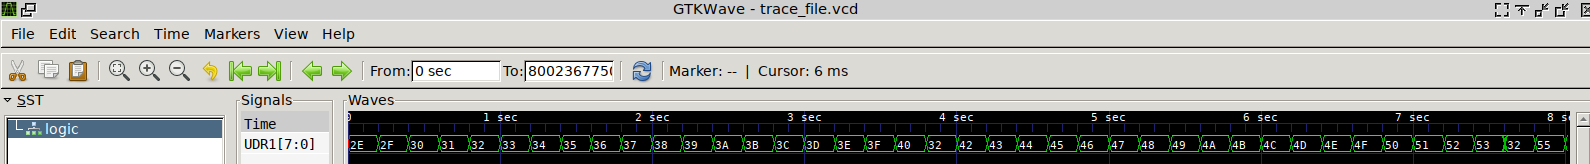
\includegraphics[width=\linewidth]{projet_sur_simavr/rs232_wave.png}
\caption{Chronogramme issu de l'ex\'ecution du code incr\'ementant \`a chaque
it\'eration de la boucle infinie l'octet transmis sur le port s\'erie.}
\label{f1}
\end{figure}

\section{\'Emulation du mat\'eriel autour du processeur}

{\tt simavr} propose un certain nombre d'exemples de circuits \'emul\'es dans
{\tt examples/} dont nous nous inspirons pour notre projet. Nous constatons que
chaque r\'epertoire contient la description d'un circuit imprim\'e avec ses 
p\'eriph\'eriques, \`a c\^ot\'e duquel est fourni le programme qui devra \^etre
flash\'e dans le microcontr\^oleur. Si par exemple nous analysons
{\tt examples/board\_timer\_64led}, nous constatons que le comportement du 
circuit imprim\'e est d\'ecrit dans {\tt timer\_64led.c} tandis que le logiciel 
\`a embarquer dans le microcontr\^oleur se trouve dans 
{\tt atmega168\_timer\_64led.c}. Ici encore les noms ont une importante, tel 
que nous le constatons en lisant le {\tt Makefile}~: il faut que le nom du 
firmware {\em soit le m\^eme que le nom du circuit}, pr\'efix\'e du nom du 
processeur support\'e, commen\c cant par {\tt atmega}. En effet dans le 
{\tt Makefile} nous constatons {\tt target=timer\_64led} et 
{\tt firm\_src=\$\{wildcard at*\$\{target\}.c\}} qui signifie de rechercher 
tous les fichiers commen\c cant par {\tt at} et contenant le nom de la cible 
qu'est le nom du circuit imprim\'e.

Ainsi, chaque r\'epertoire de projet contient deux fichiers, le firmware qui 
peut s'ex\'ecuter par {\tt run\_avr}, et un ex\'ecutable pour l'ordinateur 
h\^ote, g\'en\'eralement au format Intel x86~:
\begin{verbatim}
$ file atmega32u4_PPScontrol.axf obj-x86_64-linux-gnu/PPScontrol.elf 
atmega32u4_PPScontrol.axf:           ELF 32-bit LSB executable, Atmel AVR 8-bit, ...
obj-x86_64-linux-gnu/PPScontrol.elf: ELF 64-bit LSB pie executable, x86-64, version 1 (SYSV), ...
\end{verbatim}
Le premier fichier s'ex\'ecute sur l'\'emulateur~: 
\verb~../../simavr/run_avr atmega32u4_PPScontrol.axf~ se traduit
par la s\'equence
{\footnotesize
\begin{verbatim}
Loaded 390 .text at address 0x0
Loaded 0 .data
SIMAVR: UART INIT
SIMAVR: UART RESET
SIMAVR: IOPORT @0x25<-0x20
SIMAVR: IOPORT @0x2b<-0x4
SIMAVR: BAUDRATE 0x67
0x18.
SIMAVR: IOPORT @0x25<-0x0
/
SIMAVR: IOPORT @0x25<-0x20
0
SIMAVR: IOPORT @0x25<-0x0
1
SIMAVR: IOPORT @0x25<-0x20
2
SIMAVR: IOPORT @0x25<-0x0
\end{verbatim}
}

En effet, en l'absence de stimulation externe, ce programme se contente de 
commuter l'\'etat du port B et afficher un caract\`ere sur le port s\'erie selon
\begin{lstlisting}[language=C]
 flag_int2=0;   
 while(1)
  {transmit_data(symbole);
   if (flag_int2!=0) {transmit_data('2'); flag_int2=0;}
   PORTB^=(1<<PORTB5); // bouge PORTB 
   _delay_ms(200);
   symbole++;
  }
}
\end{lstlisting}
mais plus int\'eressant, ex\'ecuter ce m\^eme programme dans le contexte de la 
plateforme par\\
\verb~./obj-x86_64-linux-gnu/PPScontrol.elf~ se traduit par le message 
p\'eriodique contenant le symbole ``2'' transmis par le microcontr\^oleur (ici 
apr\`es le symbole ``A'') indiquant qu'une interruption mat\'erielle a \'et\'e 
d\'eclech\'ee sur le microcontr\^oleur

{\footnotesize
\begin{verbatim}
SIMAVR: IOPORT @0x25<-0x20
@
SIMAVR: IOPORT @0x25<-0x0
PPS:PD2
PD2
ICP
A2
SIMAVR: IOPORT @0x25<-0x20
B
SIMAVR: IOPORT @0x25<-0x20
\end{verbatim}
}
\noindent et par ailleurs l'\'emulation du circuit imprim\'e a aussi pris 
connaissance du d\'eclenchement de l'interruption en affichant ``PD2'' tel 
que propos\'e dans la fonction de callback li\'ee \`a ce gestionnaire 
d'interruption. En effet dans le fichier d'\'emulation du circuit imprim\'e 
{\tt PPScontrol.c}, nous trouvons
\begin{lstlisting}[language=C]
void pd2_changed_hook(struct avr_irq_t * irq, uint32_t value, void * param) {printf("PD2\n");}
...
avr_irq_t* pd2= avr_io_getirq(avr, AVR_IOCTL_IOPORT_GETIRQ('D'), 2);
avr_irq_register_notify(pd2, pd2_changed_hook, NULL);
\end{lstlisting}
\noindent tandis que le signal 1-PPS est \'emul\'e par
\begin{lstlisting}[language=C]
if (alarm_flag==1) {
  avr_raise_irq(pd2,0);
  avr_raise_irq(icp,0);
  usleep(100);
  avr_raise_irq(icp,1);
  avr_raise_irq(pd2,1);
}
\end{lstlisting}
\noindent avec {\tt alarm\_flag} un drapeau activ\'e par un signal (au sens 
Unix, {\tt man 7 signal}) qui se d\'eclenche toutes les secondes. La seconde 
occurrence de ``PD2'' correspond au front descendant car l'\'emulateur du 
circuit imprim\'e n'est pas au courant de notre configuration sur le 
micronctr\^oleur du d\'eclenchement de l'interruption sur front montant 
uniquement, tandis que ``PPS'' est un message qui indique que la condition 
d'alarme a \'et\'e atteinte. Ces deux messages sont transmis par {\tt 
PPScontrol.c} (circuit imprim\'e) et ne doivent pas \^etre confondus avec les 
messages transmis par {\tt atmega32u4\_PPScontrol.c} (firmware ex\'ecut\'e sur 
l'\'emulateur de microcontr\^oleur).

\section{Mise en \oe uvre pour la d\'etection du PPS et asservissement du quartz}

Fort de ces connaissances, nous pouvons d\'ecrire le comportement du circuit 
imprim\'e utilis\'e pour r\'ealiser le projet~: nous devons r\'eagir aux 
modifications sur la PWM qui contr\^ole la varicap, qui doit donc changer la 
fr\'equence de cadencement du microcontr\^oleur, et recevoir les impulsions 
1-PPS sur une entr\'ee timer ad\'equate. Nous ne rentrons pas dans les 
d\'etails de 
\url{https://github.com/jmfriedt/l3ep/blob/master/board_project/PPScontrol.c} 
mais c'est le r\^ole de ce fichier que de capturer ces informations et les 
restituer sur la console \`a l'utilisateur. On notera que l'\'emulation du 
1-PPS s'obtient par le m\'ecanisme des alarmes qui est classique sous unix 
mais ne permet probablement pas la compilation de ce programme sous MS-Windows. 
Si ce dernier syst\`eme d'exploitation doit \^etre utilis\'e, nous proposons
une alternative de d\'eclenchement d'un \'ev\`enement p\'eriodique gr\^ace
au {\em OpenGL utility toolkit} (GLUT)~: ce cas est un peu plus complexe
car OpenGL impose une boucle infinie pour g\'erer les \'ev\`enements li\'es
\`a l'interface graphique et la simulation du microcontr\^oleur est report\'ee
dans un {\em thread} s\'epar\'e.

Ainsi, nous compilerons {\tt PPScontrol.c} (qui ne devrait normalement pas 
avoir \`a \^etre modifi\'e, sauf erreur de description du comportement du 
circuit) qui fait appel \`a {\tt atmega32u4\_PPScontrol.c}. Nous avons fourni 
une version minimaliste de ce programme embarqu\'e pour d\'emontrer le bon
fonctionnement de l'approche, mais tout le projet reste \`a impl\'ementer, 
\`a savoir
\begin{itemize}
\item interruption {\em input capture} sur le timer 1
\item PWM sur le timer 0
\item caract\'erisation en boucle ouverte de la fr\'equence du quartz en 
fonction de la commande (virtuelle) du polarisation de la varicap. Ce point
risque d'\^etre handicap\'e par le peu de pr\'ecision du 1-PPS g\'en\'er\'e
par logiciel ... faire au mieux.
\end{itemize}

{\bf Votre travail devrait donc se limiter \`a ajouter des fonctionnalit\'es 
\`a {\tt atmega32u4\_PPScontrol.c} tandis que nous (\'Emile + JMF) nous 
chargerons de rendre l'\'emulation du circuit imprim\'e aussi r\'ealiste que 
possible dans {\tt PPScontrol.c}}

En l'absence d'un oscilloscope pour observer les signaux, profitez des traces 
pour observer l'\'etat des registres internes au processeur (dont vous ne 
pourriez m\^eme pas observer l'\'etat avec du ``vrai'' mat\'eriel dans 
certains cas).

\section{\'Emulation du timer}

Nous mentionnons en appendice \ref{tim} un cas o\`u le timer ne semble pas 
fonctionner selon nos attentes. Nous illustrons ici un cas qui semble 
fonctionner correctement~: le timer 3 est configur\'e pour d\'eclencher une 
interruption sur {\em overflow} avec un pre-scaler de 256 et sur {\em input 
capture}. Le signal d'input capture est g\'en\'er\'e environ chaque seconde. 
Nous constatons la sortie
{\footnotesize
\begin{verbatim}
SIMAVR: IOPORT @0x2e<-0x0
.........i05E2 0CDC 0002.
2....
SIMAVR: IOPORT @0x2e<-0x40
......iF1BE 05C1 0001.
2.....
SIMAVR: IOPORT @0x2e<-0x0
...
..........i98BD C1F6 0001.
2.
SIMAVR: IOPORT @0x2e<-0x40
.....
SIMAVR: IOPORT @0x2e<-0x0
..........i3DC8 4D58 0002.
2
\end{verbatim}
}
Avec un pre-scaler de 256, le timer3 en mode normal se d\'eclenche toutes les 
1,05~s. Nous constatons que ce rythme est \`a peu pr\`es respect\'e, avec
parfois deux d\'eclenchements entre deux input capture dont le signal n'a pas
pr\'etention d'exactitude. Chaque message ``SIMAVR:'' indique un changement
d'\'etat du port B (interruption overflow) et la dern\`ere valeur de chaque 
message qui suit un ``i'' (input capture) est le nombre d'overflows (1 ou 2). 
Finalement, les deux autres valeurs sont celles de ICR3 (valeur du timer au 
moment de l'input capture) et TCNT3, la diff\'erence entre les deux \'etant 
le temps de quitter l'ISR et effectuer les affichages. Ce r\'esultat est donc 
coh\'erent avec nos attentes.

De la m\^eme fa\c con, en passant le pre-scaler \`a 1, nous constatons que deux 
input capture d\'eclench\'ees par le 1-PPS \'emul\'e par le signal sont 
s\'epar\'ees de 199 \`a 248 overflows, en accord avec la th\'eorie de 
$16\cdot 10^6/65536\simeq 244$.
Nous ne pourrons donc cependant pas compter sur l'exactitude du signal pour 
fournir le 1-PPS id\'eal que devrait fournir GPS.

\begin{thebibliography}{9}
\bibitem{emu} J.-M Friedt, {\em D\'evelopper sur microcontr\^oleur sans 
microcontr\^oleur~: les \'emulateurs}, GNU/Linux Magazine France HS {\bf 103} 
(Juillet-Aout 2019), disponible \`a 
\url{http://jmfriedt.free.fr/glmf_emulateur.pdf}
\end{thebibliography}

\appendix\section{\'Emulation du timer}\label{tim}

{\bf Attention}~: il y a s\^urement des probl\`emes d'impl\'ementation de 
l'\'emulation du timer sous {\tt simavr}. Le code simple ci-dessous ne se 
comporte pas comme pr\'evu~:
\begin{lstlisting}[language=C]
#define F_CPU 16000000UL
#include <avr/io.h>
#include <avr/interrupt.h>
#include <util/delay.h>  // _delay_ms

#include "avr_mcu_section.h"     
AVR_MCU(F_CPU, "atmega32u4"); 

ISR(TIMER3_OVF_vect) {PORTE^=1<<PORTE6;}

void myicp_setup() // initialisation timer3
{TCCR3A = 1<<WGM31 | 1<<WGM30;
 TCCR3B = 1<<ICES3 | 1<<WGM33 | 1<<CS31;  // -> CS30 to fail triggering overflow
 OCR3A  = 32000;
 TIMSK3 = (1<<TOIE1);
 TIFR3  = 1<<ICF3;
}

int main(void)
{char symbole='.';
 MCUCR &=~(1<<PUD);
 DDRE |=1<<PORTE6;      // blinking LED
 myicp_setup();
 sei();
 while(1) {}
}
\end{lstlisting}

Ce programme d\'eclenche une multitude d'interruptions par overflow mais si 
nous passons le bit CS30 \`a 1 dans TCCR3B il n'y a plus d'interruption 
d\'eclench\'ee, alors que nous sommes suppos\'es avoir acc\'el\'er\'e 
l'horloge d'un facteur 8. Il serait int\'eressant de corriger ce 
dysfonctionnement de l'\'emulateur en en identifiant la cause.

Dans l'\'etat actuel de notre compr\'ehension, il {\em faut} initialiser 
l'horloge du timer par

\noindent
\verb! TCCR3B = 1<<ICES3 | 1<<WGM33 | 1<<CS30;!

\noindent
alors que 

\noindent
\verb! TCCR3B = 1<<ICES3 | 1<<WGM33 | 1<<CS31;!

\noindent
qui devrait simplement abaisser d'un facteur 8 la fr\'equence de cadencement, 
se traduit par l'absence d'incr\'ement du timer tel que observ\'e en affichant 
{\tt TCNT3}. Nous atteignons donc ici les limites de l'\'emulation, dont il 
faut corriger les dysfonctionnements.

Comme avec du vrai mat\'eriel, il faudra peut etre revenir \`a quelques 
exp\'eriences de base pour v\'erifier quel mode te timer fonctionne dans 
quelles conditions.
\end{document}
